\begin{filecontents*}[overwrite]{\jobname.bib}
  @misc{misra2019,
    author = {Rishabh Misra},
    title = {{IMDB} Spoiler Dataset},
    year = {2019},
    howpublished = {Kaggle},
    url = {https://www.kaggle.com/datasets/rmisra/imdb-spoiler-dataset}
  }
  @misc{andrezaza2023,
    author = {andrezaza},
    title = {Massive Rotten Tomatoes Movies and Reviews (version 4)},
    year = {2023},
    howpublished = {Kaggle},
    url = {https://www.kaggle.com/datasets/andrezaza/clapper-massive-rotten-tomatoes-movies-and-reviews}
  }
  @misc{leone2020,
    author = {Stefano Leone},
    title = {Rotten Tomatoes Movies and Critic Reviews Dataset},
    year = {2020},
    howpublished = {Kaggle},
    url = {https://www.kaggle.com/datasets/stefanoleone992/rotten-tomatoes-movies-and-critic-reviews-dataset}
  }
  @article{vrandecic2014,
    author = {Denny Vrande{\v{c}}i{\'c} and Markus Kr{\"o}tzsch},
    title = {Wikidata: A Free Collaborative Knowledgebase},
    journal = {Communications of the ACM},
    volume = {57},
    number = {10},
    pages = {78--85},
    year = {2014}
  }
  @misc{wdqs,
    author = {{Wikimedia Foundation}},
    title = {Wikidata Query Service},
    year = {2026},
    url = {https://query.wikidata.org},
    note = {Accessed 2026-10-14}
  }
  @misc{wikipedia,
    author = {{Wikimedia Foundation}},
    title = {English Wikipedia},
    year = {2026},
    url = {https://en.wikipedia.org},
    note = {Text licensed under CC BY-SA 4.0. Accessed 2026-10-14}
  }
  @misc{mediawikiapi,
    author = {{MediaWiki}},
    title = {MediaWiki Action API: TextExtracts and Wikibase wbgetentities},
    year = {2026},
    url = {https://www.mediawiki.org/wiki/API:Main_page},
    note = {Accessed 2026-10-14}
  }
  @inproceedings{barbaresi2021,
    author = {Adrien Barbaresi},
    title = {Trafilatura: A Web Scraping Library and Command-Line Tool for Text Discovery and Extraction},
    booktitle = {Proceedings of the 59th Annual Meeting of the Association for Computational Linguistics and the 11th International Joint Conference on Natural Language Processing: System Demonstrations},
    pages = {122--131},
    year = {2021}
  }
  @inproceedings{mckinney2010,
    author = {Wes McKinney},
    title = {Data Structures for Statistical Computing in Python},
    booktitle = {Proceedings of the 9th Python in Science Conference},
    pages = {56--61},
    year = {2010}
  }
  @misc{rfc9309,
    author = {Martijn Koster and Gary Illyes and Henner Zeller and Lizzi Sassman},
    title = {Robots Exclusion Protocol},
    howpublished = {RFC 9309},
    year = {2022}
  }
  @book{manning2008,
    author = {Christopher D. Manning and Prabhakar Raghavan and Hinrich Sch{\"u}tze},
    title = {Introduction to Information Retrieval},
    publisher = {Cambridge University Press},
    year = {2008}
  }
  @misc{rttos,
    author = {Fandango},
    title = {Rotten Tomatoes Terms of Use},
    year = {2026},
    url = {https://www.rottentomatoes.com/policies/terms-of-use},
    note = {Accessed 2026-10-09}
  }
  @misc{imdbnc,
    author = {IMDb},
    title = {{IMDb} Non-Commercial Datasets},
    url = {https://developer.imdb.com/non-commercial-datasets/}
  }
\end{filecontents*}

\documentclass[sigconf]{acmart}

\usepackage[utf8]{inputenc}
\usepackage[T1]{fontenc}
\usepackage{enumitem}
\usepackage[strings]{underscore}
\usepackage{url}
\usepackage{tabularx}

\setlength{\abovecaptionskip}{5pt}
\setlength{\belowcaptionskip}{5pt}

\title{Information Processing and Retrieval Project: PRrevIews, Searching Films by What Their Reviews Say -- Milestone 1}

\author{João Belchior}
\affiliation{%
  \institution{FEUP}
  \city{Porto}
  \country{Portugal}
}
\email{up202108777@up.pt}

\author{Catarina Guimarães}
\affiliation{%
  \institution{FEUP}
  \city{Porto}
  \country{Portugal}
}
\email{up202307420@up.pt}

\author{Sara García}
\affiliation{%
  \institution{FEUP}
  \city{Porto}
  \country{Portugal}
}
\email{up202306877@up.pt}

\author{Tiago Yin}
\affiliation{%
  \institution{FEUP}
  \city{Porto}
  \country{Portugal}
}
\email{up202306438@up.pt}

\begin{document}

\begin{abstract}
  Film reviews describe what a film is like in a way that metadata and star ratings cannot. This work prepares the data for PRrevIews, a search system that finds films through the content of their reviews and contrasts two perspectives: general audiences and professional critics. We combine audience reviews from the IMDb Spoiler Dataset with critic reviews from a Rotten Tomatoes dataset, linking the two through Wikidata identifiers. We also enrich the collection with structured film metadata and English Wikipedia article extracts. Because Rotten Tomatoes mainly provides short review quotes, we additionally recovered the full text of 56,785 critic reviews from the critics’ own websites.
\end{abstract}

\keywords{Information Retrieval, Film Reviews, Critics and Audiences, Data Integration, Web Scraping, Wikidata, Wikipedia, Exploratory Analysis}

\begin{CCSXML}
  <ccs2012>
  <concept>
  <concept_id>10002951.10003227.10003233</concept_id>
  <concept_desc>Information systems~Information retrieval</concept_desc>
  <concept_significance>500</concept_significance>
  </concept>
  </ccs2012>
\end{CCSXML}

\ccsdesc[500]{Information systems~Information retrieval}

\maketitle

\section{Introduction}
When choosing a film, we often look for what others have said about it, whether online or in person. Ratings indicate whether viewers liked a film, but reviews help explain why---for example, whether its atmosphere is sombre or cheerful, or how its cinematography compares with that of the director's other films. Reviews therefore contain rich information about films and offer multiple perspectives.

PRrevIews is a search system designed to help users find films based on what reviewers say about them. Its key feature is the distinction between reviews written by professional critics and those written by general audiences. The collection is also enriched with film-level information, including plot summaries, descriptive metadata, and extracts from English Wikipedia articles. This information provides additional context for the reviews and supports more detailed searches beyond ratings and basic film metadata.

\section{Milestone 1: Dataset Review and Selection}
The first step was to find data sources that provide rich, unstructured review text, structured data to describe and filter the films, and at least two sources that can be linked. We reviewed film-review datasets on Kaggle, IMDb's own data releases, Wikidata and Wikipedia, looking for full-text reviews that come with stable identifiers.

We selected four sources (Table~\ref{tab:sources}). The \textbf{IMDb Spoiler Dataset}~\cite{misra2019} provides long audience reviews with the IMDb identifier of each film. The \textbf{Massive Rotten Tomatoes Movies \& Reviews} dataset~\cite{andrezaza2023} (``Clapper'') provides critic reviews and film metadata, but uses Rotten Tomatoes identifiers. \textbf{Wikidata}~\cite{vrandecic2014, wdqs} bridges the two through its IMDb ID and Rotten Tomatoes ID properties, and also names the English Wikipedia article about each film. \textbf{English Wikipedia}~\cite{wikipedia} provides that article, a long encyclopedic description of the film, downloaded through the MediaWiki API~\cite{mediawikiapi}. The IMDb Spoiler Dataset is the anchor of the collection: its 1,572 films define which films are included. It has no title field, so titles come from Rotten Tomatoes.

\begin{table*}[t]
  \centering
  \caption{Selected data sources}
  \label{tab:sources}
  \small
  \begin{tabularx}{\textwidth}{lXXXX}
    \toprule
    & \textbf{IMDb Spoiler Dataset} & \textbf{Clapper (Rotten Tomatoes)} & \textbf{Wikidata} & \textbf{English Wikipedia} \\
    \midrule
    Role & Audience reviews (long text), film details & Critic reviews (short quotes, links to full reviews), film metadata & Links IMDb and Rotten Tomatoes identifiers; names each film's article & Encyclopedic description of each film (full article) \\
    Version & Kaggle v1, updated 2019-05-22 & Kaggle v4, updated 2023-04-13 & Queried 2026-10-14 & Revisions of 2026-10-14; revision IDs kept \\
    Volume & 573,913 reviews of 1,572 films & 1,444,963 reviews of 69,263 films; 143,258 film records & 90,761 IMDb $\leftrightarrow$ Rotten Tomatoes pairs; titles for 1,537 items & 1,507 articles for 1,508 linked films \\
    \bottomrule
  \end{tabularx}
\end{table*}

Some alternatives were discarded. The Rotten Tomatoes dataset by Leone~\cite{leone2020} was used first and replaced: like Clapper, it only contains short quotes of the critics' reviews, but it has no link to each review's full text, while Clapper has one for 85\% of its reviews and linked more of our films (1,506 against 1,442). The IMDb Non-Commercial Datasets~\cite{imdbnc} were dropped because their metadata is already covered by the two Kaggle datasets. Scraping Rotten Tomatoes directly was rejected, since its Terms of Use forbid any automated collection~\cite{rttos}.

\section{Selection of Suitable Subsets}
\label{sec:subsets}
The full sources hold about 1.9 million reviews, most of them about films outside our scope. The collection is restricted to the films of the IMDb Spoiler Dataset: of its 1,572 films, 1,514 link to a Rotten Tomatoes film through Wikidata (many in IMDb are not actually films but tv shows and some have no matching ID between them), 1,508 of these have a titled Rotten Tomatoes page, and \textbf{1,492} keep at least one critic review after cleaning. Wikipedia articles are downloaded for the 1,508 linked films; 1,491 of the final films have one.

Even for these films, the collection would hold 756,730 reviews without limits. Popular films such as blockbusters would dominate, and the raw files need a large amount of memory, which would also slow down later tasks. We decided to cap the reviews \textbf{per film and per source} at 200 (Table~\ref{tab:cap}). Within a capped film, reviews are chosen at random with a fixed seed, keeping the original mix of opinions.

\begin{table}[h]
  \centering
  \caption{Collection size for different caps (1,492 films)}
  \label{tab:cap}
  \small
  \begin{tabular}{lrrr}
    \toprule
    Cap per film & Audience & Critics & Total \\
    \midrule
    50 & 73,529 & 66,880 & 140,409 \\
    100 & 142,290 & 115,482 & 257,772 \\
    \textbf{200 (chosen)} & \textbf{259,139} & \textbf{179,018} & \textbf{438,157} \\
    No cap & 548,957 & 207,773 & 756,730 \\
    \bottomrule
  \end{tabular}
\end{table}

Rotten Tomatoes only provides short quotes, median 21 words, against a median of 189 words for IMDb reviews. To give critics comparable text, we followed each review's link to the critic's website (Section~\ref{sec:scraping}). The full crawl recovered a third of the reviews with a link. The texts are unevenly spread: critic reviews of 2010s films have a much higher chance of having a full text than those of 2000s films, and some publications are almost entirely missing while others are nearly complete.

\section{Data Authority and Quality Assessment}
\textbf{Authority.} IMDb is the largest public film-review community, and the IMDb Spoiler Dataset was collected from it for research, in a single stable version; its reviews are self-selected and stop in 2018. Rotten Tomatoes only lists reviews from approved critics and publications, but Clapper is a third-party scrape, so its license is the uploader's own declaration. Wikidata is community-curated and openly licensed, but changes over time, so results depend on the query date. Wikipedia is written by its community under editorial policies (neutral point of view, verifiable sources); its articles change continuously, so the revision ID of each one is stored. The scraped full reviews are original, copyrighted articles: they are used only for research within the project and are not redistributed.

\textbf{Quality.} We profiled every raw file with an inspection step that reports, for each column, the missing values, distinct values and most frequent values. The main issues are summarised below; the full list is in Table~\ref{tab:quality} (annex).
\begin{itemize}[leftmargin=*]
  \item \textbf{Duplicates and empty texts:} 12,394 duplicate and 69,225 empty Rotten Tomatoes reviews; 429 IMDb reviews repeat another review of the same film.
  \item \textbf{Placeholders:} quotes such as ``Parental Content Review'' or ``Click to read review'' that are not reviews.
  \item \textbf{Fake and misleading dates:} 48,083 reviews are dated \texttt{2000-01-01}, and critic dates record when a review was \textit{added} to Rotten Tomatoes (about 19\% are more than five years after the film's release).
  \item \textbf{Inconsistent formats:} critic scores in 1,701 formats (\texttt{3/5}, \texttt{B+}\ldots), HTML codes such as \texttt{\&\#44;} in quotes, IMDb dates written in words and durations such as \texttt{1h 44min}.
  \item \textbf{Spoilers and critic opinions in Wikipedia:} articles tell the plot, ending included, and many summarise the critics' reception, so they are kept only in the film documents.
\end{itemize}

\section{Data Processing Pipeline}
The whole collection and preparation process was designed as a \textbf{reproducible and modular pipeline} (Figure~\ref{fig:pipeline}).  It is implemented in \texttt{Python} with the \texttt{pandas}~\cite{mckinney2010} and \texttt{trafilatura}~\cite{barbaresi2021} libraries, and a \texttt{makefile} automates every step. The stages run in a straight line, each one a \texttt{make} target with its own module and output folder. Downloads need no credentials and happen only once, failed or cut-off downloads are deleted instead of being mistaken for finished files. All Python packages are pinned to the versions we ran.

\begin{figure}[t]
  \centering
  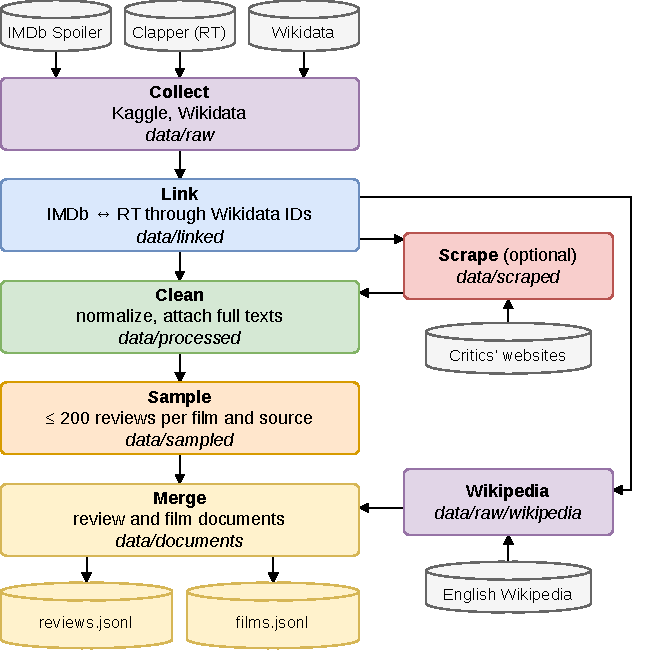
\includegraphics[width=\columnwidth]{pipeline_vertical.pdf}
  \caption{Data processing pipeline.}
  \Description{Flow diagram of the pipeline: three sources go through collect, link, clean, sample and merge, producing reviews.jsonl and films.jsonl; scraping and Wikipedia are side branches.}
  \label{fig:pipeline}
\end{figure}

\subsection{Collection}
Collection is done by the \texttt{makefile} and one small module: the Kaggle datasets are downloaded with \texttt{curl} from Kaggle's public endpoint, pinned to their versions, and unzipped into \texttt{data/raw}. The links come from a SPARQL query to the Wikidata Query Service, which keeps items with an IMDb title ID and a Rotten Tomatoes movie ID. The query reads every Rotten Tomatoes ID, not only the current one, because Clapper still uses some IDs that Wikidata now marks as outdated. It takes 8--16 seconds; asking for the films' titles or their Wikipedia articles in the same query pushed it past Wikidata's 60-second limit, so the Wikipedia titles are fetched separately from the Wikidata API by \texttt{data_wikipedia_titles.py}.

\subsection{Linking}
Linking (\texttt{data_link.py}) runs \textbf{before} cleaning because identifiers must be fixed before films can be matched, and restricting the data to our films first means every later stage processes only the subset of reviews of our films instead of the whole thing. The stage removes the stray \texttt{/} from two IMDb IDs and the \texttt{m/} prefix from Rotten Tomatoes IDs, keeps a link only when the IMDb film is one of ours and its Rotten Tomatoes page exists in Clapper with a title, attaches the IMDb ID to the matching critic reviews and film rows, and adds each film's Wikipedia title. The links are one-to-one and the IMDb review identifiers match the film identifiers exactly.

\subsection{Wikipedia Articles}
The Wikipedia module (\texttt{data_wikipedia.py}) downloads the English Wikipedia article of every linked film through the MediaWiki API, as plain text, with its address, page ID and revision ID, following redirects to renamed articles. Since an article tells the plot, ending included, and summarises the critics, it is stored only in the film documents, with its section headings kept so that sections can be left out at indexing time.

\subsection{Full-Text Scraping}
\label{sec:scraping}
The scraper (\texttt{data_scrape.py}) reads the linked critic reviews and follows each review's link to the critic's website. It waits at least 2 seconds between requests to the same site, skips sites asking for more than 60 seconds. Each of its 32 workers crawls a whole site, so a slow site only occupies its own worker, and the article text is extracted with \texttt{trafilatura}. A page counts as a full review only if it has at least 150 words of article and contains 6 consecutive words of the Rotten Tomatoes quote, which rejects homepages and redirects. The crawl ran for about 10 hours and recovered \textbf{56,838 full reviews} (Table~\ref{tab:crawl}, annex).

\subsection{Cleaning}
The cleaning module (\texttt{data_clean.py}) decodes HTML codes, removes duplicates, empty texts and placeholders, moves the ``[Full review in Spanish]'' tags of translated quotes into a \texttt{translated} flag, sets fake dates to unknown, converts fractions and letter grades into a 0--1 \texttt{score}, converts IMDb dates to \texttt{YYYY-MM-DD} and durations to minutes, and splits genres, directors and writers into lists. Scraped pages are attached as full texts only if their quote check passes, also after decoding HTML codes, with leftover layout borders removed.

\subsection{Sampling}
The sampling module (\texttt{data_sample.py}) applies the selection of Section~\ref{sec:subsets}: it keeps the 1,492 films with both perspectives and at most 200 reviews per film and source, preserving each film's mix of opinions and taking critic reviews with a full text first.

\subsection{Document Building}
The merge module (\texttt{data_merge.py}) renames every field, chooses each critic review's text (the full review when there is one, otherwise the quote), copies the main film details into each review, and writes \texttt{reviews.jsonl} (438,157 documents) and \texttt{films.jsonl} (1,492 documents, with their Wikipedia articles), the final product of the pipeline.

\section{Conceptual Domain Model}
Figure~\ref{fig:uml} shows the conceptual model of the collection. Its central entity is the \textbf{review}, an abstract class that is always about one \textbf{movie} and written by one \textbf{reviewer}.

\begin{figure}[!htb]
  \centering
  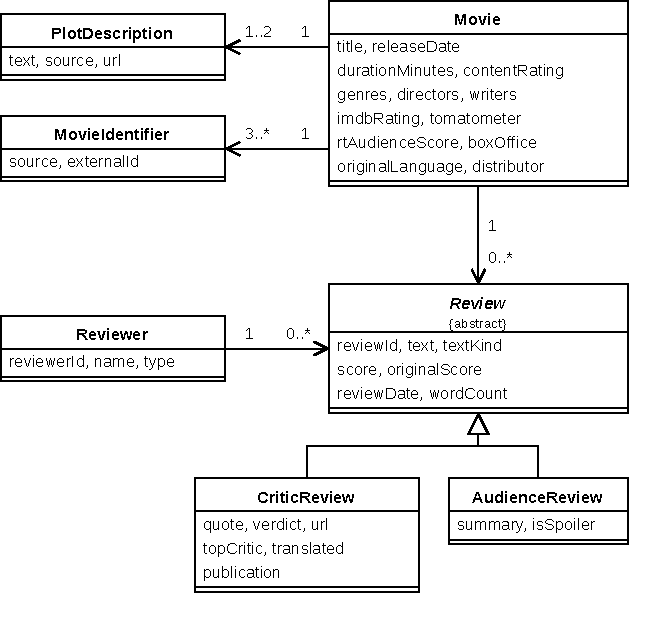
\includegraphics[width=\columnwidth]{domain_model_small.pdf}
  \caption{UML class diagram of the PRrevIews data domain.}
  \Description{UML class diagram}
  \label{fig:uml}
\end{figure}

\section{Exploratory Analysis and Collection Characterization}
\label{sec:eda}
The final collection holds 1,492 films and 438,157 review documents, with 121.8 million words of review text. The films were released between 1921 and 2018 (median 2003), most of them in the 1990s--2010s, and the most common genres are Drama (754), Comedy (504) and Action (419). The figures below are produced by the last stage of the pipeline (\texttt{data_analysis.py}).

\textbf{Critics versus audiences.} Comparing each film's Tomatometer with its audience score (Figure~\ref{fig:gap}), audiences rate films 5.1 points higher on average, and large disagreements are mostly one-sided: audiences rate \textbf{188 films at least 25 points higher} than critics, while critics do so for only 34. The largest gaps are \textit{Grandma's Boy} (Tomatometer 15, audience 85), \textit{Drop Dead Fred} (11 vs.\ 77) and \textit{The Boondock Saints} (27 vs.\ 91), which are exactly the films of our first information need.

\textbf{Review text.} Critic full texts (median 738 words) are about four times longer than audience reviews (186), while the quotes are very short (20), so retrieval will need length normalization~\cite{manning2008}; the 593 critic texts over 5,000 words are mostly pages covering several films (Figure~\ref{fig:lengths}, annex). The two perspectives also use different words (Figure~\ref{fig:words}, annex): critic quotes favour genre and craft terms such as \textit{thriller}, \textit{filmmaking} and \textit{cinematic}, while audiences describe their own viewing with words such as \textit{movie}, \textit{watch}, \textit{think} and \textit{acting}.

\textbf{Opinions and film text.} Audience ratings are polarized, with peaks at 10 and at 1 (mean 7.0/10; Figure~\ref{fig:ratings}, annex), and 69.1\% of critic reviews are fresh (Table~\ref{tab:perspectives}, annex). The film documents add 5.3 million words of Wikipedia text (median 2,799 words per article).

\begin{figure}[h]
  \centering
  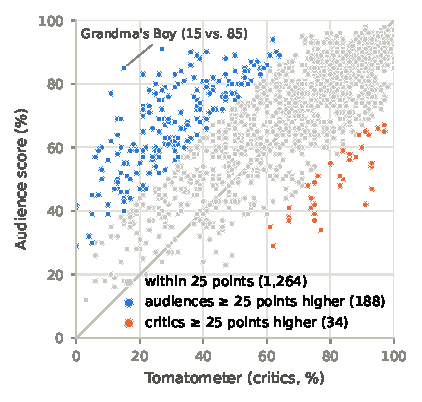
\includegraphics[width=\columnwidth]{figs/critics_vs_audiences.pdf}
  \caption{Tomatometer versus audience score for the 1,486 films with both scores. Audiences rate 188 films at least 25 points higher than critics; critics do so for 34.}
  \Description{Scatter plot of critic and audience scores per film: most films lie near the diagonal, a large group lies well above it (audiences much higher) and a small group well below it.}
  \label{fig:gap}
\end{figure}

\section{Definition and Characterization of Documents in the Final Collection}
Each document is \textbf{one review}, critic or audience, carrying a copy of its film's main details, so that it can be searched, filtered and shown on its own; a separate file holds one document per film, including its Wikipedia article, which is not copied into the reviews. Every document has the following fields (Table~\ref{tab:fields}, annex). We validated every document: all IDs are unique, no text is empty, scores and dates are well formed, every film has a title and both perspectives, and the film details in each review match the film file.

\section{Potential Research Tasks}
Based on the exploratory analysis and the structure of the documents, we identify the following information needs. These tasks focus on information expressed in review text rather than on simple title or rating searches.

\begin{enumerate}[leftmargin=*]
  \item \textbf{Audience--critic disagreement:} Find films that audiences defended despite negative critical reviews.

    Example query: \emph{audiences liked the film although critics disliked it}.

  \item \textbf{Themes and atmosphere:} Find films whose reviews describe themes such as grief, isolation, or emotional recovery.

    Example query: \emph{films about grief and loneliness with a hopeful ending}.

  \item \textbf{Strengths and weaknesses:} Find films praised for their acting or cinematography but criticized for their pacing or plot.

    Example query: \emph{great acting but slow pacing}.

  \item \textbf{Perspective comparison:} Find films where critics and audiences have different opinions about the story, visuals, or performances.

    Example query: \emph{critics praised the visuals but audiences found the story confusing}.

  \item \textbf{Plot and setting:} Find films described through their plot or setting, even when the query does not mention a specific title or genre.

    Example query: \emph{film set in an isolated and hostile environment}.
\end{enumerate}

\section{Conclusion and Future Work}
This first milestone produced a reproducible collection of 438,157 film reviews about 1,492 films, combining the audience and critic perspectives through Wikidata identifiers, describing them with their Wikipedia articles, and recovering 56,785 full critic reviews from the critics' own websites. After a one-time download, a single \texttt{make} command rebuilds the collection in about two minutes with identical results. Its main limitations are that 68\% of critic documents still carry only a short quote, unevenly across film eras and publications, that critic dates record when a review was added to Rotten Tomatoes, and that the Wikipedia articles contain spoilers and critic summaries. Future work includes a length limit for scraped texts, choosing which Wikipedia sections to index, fuller keyword extraction and named-entity recognition, and the indexing and retrieval work of Milestone~2.

\clearpage

\bibliographystyle{ACM-Reference-Format}
\bibliography{\jobname}

\section{Annexes}
\suppressfloats[t]

\begin{table}
  \centering
  \caption{Outcome of the crawl (174,305 reviews with a link)}
  \label{tab:crawl}
  \small
  \begin{tabular}{lrr}
    \toprule
    Result & Reviews & Share \\
    \midrule
    \textbf{Full review (quote confirmed)} & \textbf{56,838} & \textbf{32.6\%} \\
    Page gone (404/410) & 29,586 & 17.0\% \\
    Blocked by \texttt{robots.txt} & 20,471 & 11.7\% \\
    Text found, quote not matched & 18,460 & 10.6\% \\
    Site unreachable & 18,070 & 10.4\% \\
    No article text & 14,872 & 8.5\% \\
    Refused, rate-limited or other errors & 16,008 & 9.2\% \\
    \bottomrule
  \end{tabular}
\end{table}

\begin{table}
  \centering
  \caption{Entities of the domain model}
  \label{tab:entities}
  \small
  \begin{tabularx}{\columnwidth}{lX}
    \toprule
    Entity & Source and content \\
    \midrule
    Film & IMDb (plot, dates, duration, rating, genres), Rotten Tomatoes (title, scores, age rating, language), Wikidata (ID) \\
    Audience review & IMDb: text, summary, rating 1--10, spoiler flag \\
    Critic review & Rotten Tomatoes and critics' websites: quote, verdict, scores, flags, link, full text \\
    User, Critic, Publication & Authors of the reviews \\
    Genre, Person & Genres; directors and writers \\
    Wikipedia article & English Wikipedia, through Wikidata: title, address, revision ID, full text (one per film) \\
    Film--Film & Remakes and adaptations (future, Wikidata) \\
    \bottomrule
  \end{tabularx}
\end{table}

\begin{table}
  \centering
  \caption{Audience and critic reviews}
  \label{tab:perspectives}
  \small
  \begin{tabularx}{\columnwidth}{lXX}
    \toprule
    & Audience & Critics \\
    \midrule
    Per film & median 200 (min 11) & median 126 (min 1) \\
    Authors & 131,034 users & 6,062 critics, 1,819 publications \\
    Opinion & mean 7.00/10 & 69.1\% fresh; mean score 0.67 \\
    Dates & 1998--2018 & 1927--2023; 12,091 unknown \\
    Other & 25.1\% spoilers & 28.5\% top critics \\
    \bottomrule
  \end{tabularx}
\end{table}

\begin{figure}
  \centering
  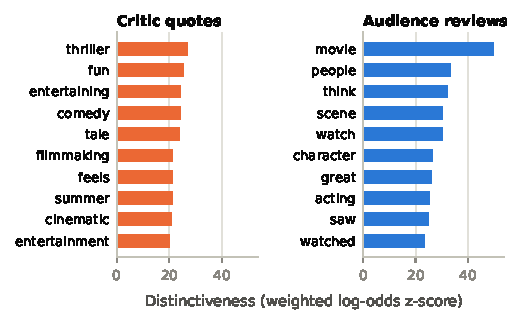
\includegraphics[width=\columnwidth]{figs/distinctive_words.pdf}
  \caption{Words most typical of critic quotes and of audience reviews (weighted log-odds z-score, critic quotes against a sample of audience reviews).}
  \Description{Two bar charts: critic quotes favour genre and craft words such as thriller, filmmaking and cinematic; audience reviews favour personal viewing words such as movie, think, watch and acting.}
  \label{fig:words}
\end{figure}

\begin{figure}
  \centering
  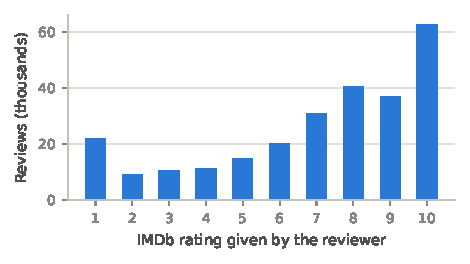
\includegraphics[width=\columnwidth]{figs/audience_ratings.pdf}
  \caption{Distribution of the 1--10 ratings given by audience reviewers.}
  \Description{Bar chart of audience ratings from 1 to 10, with the highest peak at 10 and a second peak at 1.}
  \label{fig:ratings}
\end{figure}

\begin{table*}
  \centering
  \caption{Data quality issues and their handling}
  \label{tab:quality}
  \small
  \begin{tabularx}{\textwidth}{lXX}
    \toprule
    Issue & Evidence & Handling \\
    \midrule
    Duplicate rows & 12,394 Rotten Tomatoes reviews; 1,204 Rotten Tomatoes films & Removed \\
    Empty or placeholder texts & 69,225 empty reviews; quotes such as ``Parental Content Review'' (236) or ``Click to read review'' (39) & Removed (205 placeholders in the linked reviews) \\
    Fake dates & \texttt{2000-01-01} appears 48,083 times & Set to unknown\\
    Inconsistent scores & 435,218 missing; 1,701 formats (\texttt{3/5}, \texttt{3/4}, \texttt{B+}\ldots) & New 0--1 \texttt{score} from fractions and letter grades \\
    Redundant column & \texttt{scoreSentiment} identical to \texttt{reviewState} & Dropped \\
    HTML codes & About 2,550 quotes, e.g. \texttt{\&\#44;} & Decoded \\
    Translated quotes & About 3,500 quotes end with ``[Full review in Spanish]'' & Tag removed, \texttt{translated} flag added \\
    Missing or generic links & 210,925 missing; some point to homepages (782 reviews to one) & Quote only; rejected by the quote check \\
    IMDb repeated texts & 429 reviews repeat another review of the same film & Removed \\
    IMDb formats & Dates in words, durations as \texttt{1h 44min}, two IDs ending in \texttt{/} & Converted and fixed \\
    IMDb synopsis & \texttt{plot_synopsis} missing for 233 films, median 1,260 words, describes the ending & Dropped; \texttt{plot_summary} kept \\
    Slow Wikidata query & Adding the films' Wikipedia articles took a lot of time, then was cut off & Titles fetched from the Wikidata API instead \\
    Spoilers and critic opinions & Wikipedia plots tell the ending & Kept only in the film documents; headings kept \\
    \bottomrule
  \end{tabularx}
\end{table*}

\begin{table*}
  \centering
  \caption{Fields of a review document}
  \label{tab:fields}
  \small
  \begin{tabularx}{\textwidth}{lXX}
    \toprule
    Field & Audience review & Critic review \\
    \midrule
    \texttt{id} & \texttt{imdb_<film>_<user>} & \texttt{rt_<reviewId>} \\
    \texttt{perspective} & \texttt{audience} & \texttt{critic} \\
    \texttt{text}, \texttt{text_kind} & the review (\texttt{full}) & the full review (56,637) or the quote (122,381) \\
    \texttt{quote}, \texttt{summary} & the review's title (\texttt{summary}) & the Rotten Tomatoes quote (\texttt{quote}) \\
    \texttt{score}, \texttt{original_score} & rating / 10; e.g. \texttt{8/10} & 0--1 score when understood; as written by the critic \\
    \texttt{verdict} & & \texttt{fresh} or \texttt{rotten} \\
    \texttt{is_spoiler} & true / false & \\
    \texttt{top_critic}, \texttt{translated} & & true / false \\
    \texttt{author}, \texttt{publication} & IMDb user ID & critic name; publication name \\
    \texttt{date} & date written & date added to Rotten Tomatoes \\
    \texttt{url} & & link to the full review \\
    \texttt{word_count} & words in \texttt{text} & words in \texttt{text} \\
    \texttt{film_*} & \multicolumn{2}{l}{IMDb and Wikidata IDs, title, year, genres, plot summary, IMDb rating, Tomatometer and audience score} \\
    \bottomrule
  \end{tabularx}
\end{table*}

\begin{figure*}
  \centering
  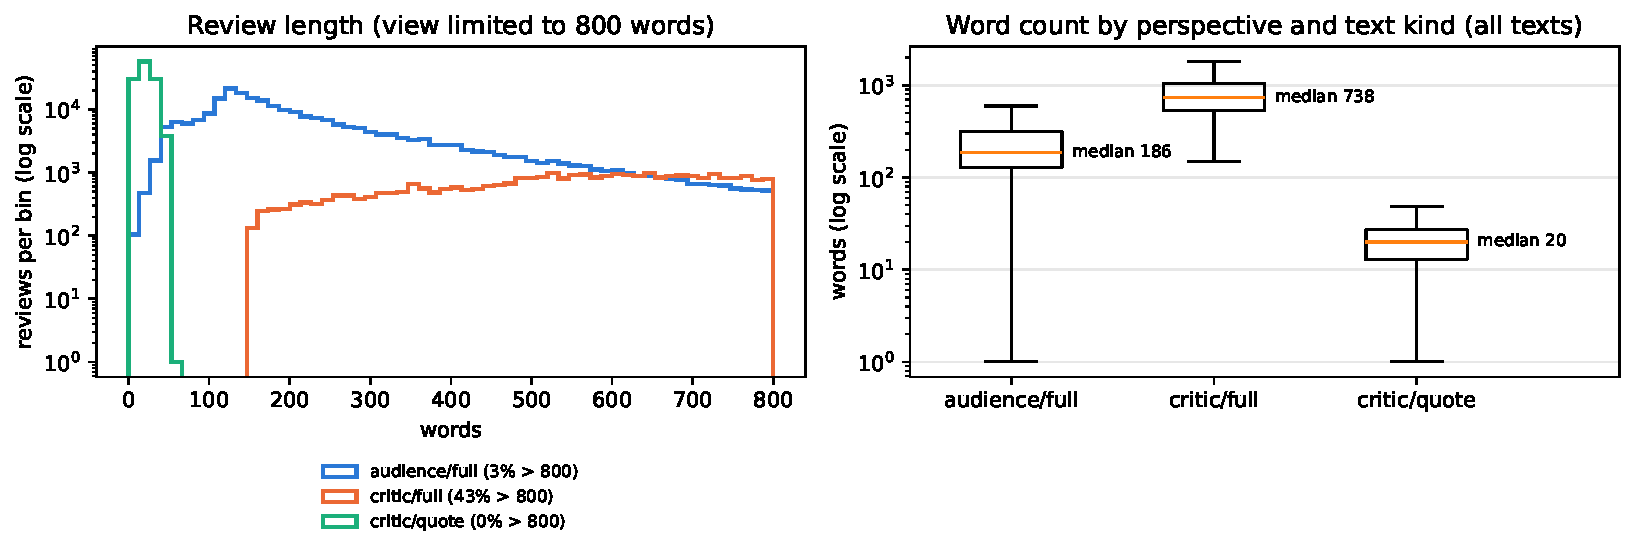
\includegraphics[width=\textwidth]{figs/text_length.pdf}
  \caption{Review length by perspective and text kind: histogram up to 800 words (left) and word counts over all texts (right, log scale).}
  \Description{Histogram and box plots of review lengths: critic quotes are around 20 words, audience reviews around 186 and critic full texts around 738.}
  \label{fig:lengths}
\end{figure*}

\end{document}
